\documentclass[a4paper, 11pt]{article}
\usepackage[utf8]{inputenc}
\usepackage{amsmath}
\usepackage{vhistory}
\usepackage{amsfonts}
\usepackage{mathtools}
\usepackage{float}
\usepackage{blindtext}
\usepackage[inline]{enumitem}
\usepackage{xcolor}
\usepackage{amsmath}
\usepackage{array}
\usepackage{listings}
\usepackage{svg}
\usepackage{color}
\usepackage{booktabs}
\usepackage{caption}
\usepackage{varioref}
\usepackage{hyperref} 
\usepackage[ruled,vlined]{algorithm2e}
\usepackage[section]{placeins}
\usepackage{comment} % enables the use of multi-line comments (\ifx \fi) 
\usepackage{graphicx}
\usepackage{lipsum} %This package just generates Lorem Ipsum filler text. 
\usepackage{fullpage} % changes the margin
\usepackage{cleveref}
\definecolor{dkgreen}{rgb}{0,0.6,0}
\definecolor{gray}{rgb}{0.5,0.5,0.5}
\definecolor{mauve}{rgb}{0.58,0,0.82}
%Includes "References" in the table of contents
\usepackage[nottoc]{tocbibind}

\DeclareMathOperator*{\argmax}{argmax} % thin space, limits underneath in displays

\newenvironment{conditions}
{\par\vspace{\abovedisplayskip}\noindent\begin{tabular}{>{$}l<{$} @{${}={}$} l}}
	{\end{tabular}\par\vspace{\belowdisplayskip}}

\renewcommand{\lstlistingname}{Algorithm}% Listing -> Algorithm
\renewcommand{\lstlistlistingname}{List of \lstlistingname s}% List of Listings -> List of Algorithms
\crefname{listing}{algorithm}{algorithms}  
\Crefname{listing}{Algorithm}{Algorithms}

\lstset{frame=tb,
	language=Python,
	aboveskip=3mm,
	belowskip=3mm,
	showstringspaces=false,
	columns=flexible,
	basicstyle={\small\ttfamily},
	numbers=left,
	numberstyle=\tiny\color{gray},
	keywordstyle=\color{blue},
	commentstyle=\color{dkgreen},
	stringstyle=\color{mauve},
	breaklines=true,
	breakatwhitespace=true,
	tabsize=3,
	inputencoding=latin1
}

%\setlength{\belowcaptionskip}{-10pt}
\makeatletter
\renewcommand{\paragraph}{%
	\@startsection{paragraph}{4}%
	{\z@}{1.0ex \@plus 1ex \@minus .2ex}{-1em}%
	{\normalfont\normalsize\bfseries}%
}
\makeatother

\usepackage{pgfplots}
\usepackage{tikz}
\usepackage{varwidth}
\usepgfplotslibrary{fillbetween}
\usetikzlibrary{calc,trees,positioning,arrows,chains,shapes.geometric,%
	decorations.pathreplacing,decorations.pathmorphing,shapes,%
	matrix,shapes.symbols}

\tikzstyle{object} = [rectangle, rounded corners, minimum width=3cm, minimum height=1cm,text centered, draw=white]
\tikzstyle{element} = [rectangle, rounded corners, minimum width=3cm, minimum height=1cm,text centered, draw=black]
\tikzstyle{xor} = [diamond, minimum width=1cm, minimum height=1cm, text centered, draw=black]
\tikzstyle{arrow} = [thick,->,>=stealth]

\pgfplotsset{width=\textwidth, height=\textheight*0.33,compat=newest}

\definecolor{train_color_1}{HTML}{8b402a}
\definecolor{train_color_2}{HTML}{e45e2d}
\definecolor{train_color_3}{HTML}{ef9c49}
\definecolor{train_color_4}{HTML}{fdea6f}

\definecolor{test_color_1}{HTML}{192574}
\definecolor{test_color_2}{HTML}{2e62a1}
\definecolor{test_color_3}{HTML}{43a7cb}
\definecolor{test_color_4}{HTML}{9ed5cd}

\pgfplotscreateplotcyclelist{train}{
	semithick,train_color_1\\%
	semithick,train_color_2\\%
	semithick,train_color_3\\%
	semithick,train_color_4\\%
}

\pgfplotscreateplotcyclelist{test}{
	semithick,test_color_1\\%
	semithick,test_color_2\\%
	semithick,test_color_3\\%
	semithick,test_color_4\\%
}



\captionsetup[figure]{skip=0pt}


\begin{document}
	%Header-Make sure you update this information!!!!
	\noindent
	\large\textbf{A Study of Reinforcement Learning} \hfill \textbf{Report DDPG} \\
	\normalsize Prof. Pietro Michiardi - Eurecom \hfill   Piero Macaluso\\
	\normalsize Prof. Elena Baralis - Politecnico di Torino  \hfill Version: \vhCurrentVersion \space from \vhCurrentDate
	
	\tableofcontents
	\newpage
	\begin{versionhistory}
		\vhEntry{1.0}{April, 16 2019}{PM}{- Created.
			
			- Added DDPG description and implementation.
			
			- Added Environments Description
			
			- Added Uniform/Prioritized Replay implementation and simulation.}
		%\vhEntry{1.1}{23.01.04}{DP|JPW}{correction}
		%\vhEntry{1.2}{03.02.04}{DP|JPW}{revised after review}
	\end{versionhistory}
	\newpage
	
	\section{Introduction} \label{introduction}
		
	The path of my master thesis began with a study of the foundations of Reinforcement Learning through a series of video lectures and slides of the course \footnote{The website of the course: \url{http://www0.cs.ucl.ac.uk/staff/d.silver/web/Teaching.html}} held by prof. David Silver and reading some chapters from \cite{sutton2018reinforcement}. 
	
	Time was spent on the implementation of some algorithms presented in the video lectures to better understand the theory and to get started with the Reinforcement Learning framework \textbf{OpenAI Gym} \cite{brockman2016openai}. This is the framework that will be used to implement the project of my thesis.
	
	In the last weeks, the main focus was on a more careful and accurate analysis of the paper \cite{kendall2018learning} from which the development of the thesis starts, and the references it contains, including the paper about \textbf{Deep Deterministic Policy Gradient algorithm (DDPG)} \cite{lillicrap2015continuous}.
	Starting from these, my main goal was to implement the DDPG in  Python along the lines of the one present in \cite{kendall2018learning} and \cite{lillicrap2015continuous} so that it can be tested, in an initial stage, with an environment less complex provided by the framework \cite{brockman2016openai}.
	
	The aim of this report is to show a background of the algorithm, the performances obtained and possible future developments.
	
	\section{Deep Deterministic Policy Gradient} \label{ddpg}
	\subsection{Application Field}
	This algorithm can be applied to situations that can not be solved using \textbf{DQN} algorithm \cite{mnih2015human} because of the presence of a continuous action spaces. A finely discretization of the action space to adapt the situation to DQN would lead to an explosion in the number of discrete actions and to the curse of dimensionality.
	
	DDPG is an algorithm which uses deep function approximators in order to learn policies in high-dimensional, continuous action spaces and it is:
	
	\begin{enumerate}[label={\alph*)},font={\color{black}\bfseries}, nolistsep]
		\item \textbf{Model-Free}: it has no prior knowledge about model, transitions or rewards;
		\item \textbf{Off-Policy}: the policy is learnt from experiences sampled from another policy;
		\item \textbf{Actor-Critic}: alternation between a policy evaluation and a policy improvement step.
	\end{enumerate}
	
	\textbf{Bellman equation} and \textbf{Q-learning} are fundamental parts of this algorithm.	It concurrently learns a Q-value function and a policy: it uses off-policy data and the Bellman equation to learn the Q-value function, and uses the Q-value function to learn the policy.
	
	Usually, in Reinforcement Learning, if the optimal action-value function $Q^*(s,a)$ is known, then in any given state, the optimal action $a^*(s)$ can be found by solving \[a^*(s) = \arg \max_a Q^*(s,a)\]
	
	When the number of discrete actions is finite, calculating the $\max$ poses no problem, because the Q-values can be calculated for each action separately, then directly compared. But when the action space is continuous, this process become highly non-trivial: it would need to be run at every steps of the episode, whenever the agent wants to take an action in the environment and this can not work.
	
	Because the action space is continuous, the function $Q^*(s,a)$ is presumed to be differentiable with respect to the action argument. For this reason, an efficient, gradient-based learning rule for a policy $\mu(s)$ which exploits that fact can be set up, approximating it with $\max_a Q(s,a) \approx Q(s,\mu(s))$.
	
	\subsection{Key Points}
	\subsubsection{Reinforcement Learning Setup}
	The Reinforcement Learning Setup is the standard one. It consists of an agent interacting with an environment $\mathit{E}$ in discrete timesteps. At each timestep $t$ the agent receives an \textbf{observation} $x_t$, takes an \textbf{action} $a_t$ and receives a scalar \textbf{reward} $r_t$. In this specific case, the actions are real-valued $a_t \in \mathbb{R}^\mathit{N}$ and it is assumed that the environment is fully-observed so $s_t = x_t$.
	
	The agent’s behavior is defined by a policy $\pi : \mathcal{S} \rightarrow \mathcal{P}(\mathcal{A})$ which maps states to a probability distribution over the actions.
	The problem is modeled as a \textbf{Markov decision process} with a state space $\mathcal{S}$, action space $\mathcal{A} = \mathbb{R}^N$, an initial state distribution $p(s_1)$, transition dynamics $p(s_{t+1}|s_t,a_t)$, and reward function $r(s_t,a_t)$.
	
	The return is defined as the sum of discounted future reward $R_t=\sum_{i=t}^{T}\gamma^{(i-t)}r(s_i,a_i)$ with a discounting factor $\gamma \in [0,1]$ and depends on the actions chosen, and therefore on the policy $\pi$.
	
	The goal in reinforcement learning is to learn a policy which maximizes the expected return from the start distribution $J=\mathbb{E}_{r_i,s_i\sim E,a_i\sim \pi}[R_1]$.  We denote the discounted state visitation distribution for a policy $\pi$ as $\rho^\pi$.
	
	\subsubsection{Learning Equations}
	
	One of the fundamental function in Reinforcement Learning, which is used also in DDPG, is the \textbf{action-value function}. It describes the expected return after taking an action $a_t$ in state $s_t$ and thereafter following policy $\pi$:
	\begin{equation}\label{eq1:actionvalue}
	Q^\pi(s_t, a_t) = \mathbb{E}_{r_i\geq t,s_{i} > t \sim \mathit{E}, a_i > t \sim \pi}[R_t|s_t,a_t]
	\end{equation}
	DDPG exploits also the \textbf{Bellman equation} which is given by
	\begin{equation}\label{eq2:bellman1}
	Q^\pi(s_t, a_t) = \mathbb{E}_{r_t,s_{t+1}\sim \mathit{E}}[r(s_t, a_t) + \gamma \mathbb{E}_{a_{t+1}\sim \pi}[Q^\pi(s_{t+1}, a_{t+1})]]
	\end{equation}
	where $s_{t+1}\sim \mathit{E}$ means that the next state is sampled from the environment $E$ and $a_{t+1}\sim \pi$ shows that the next action is taken following the policy $\pi$. If this policy is deterministic we can describe it as a function $ \mu : \mathcal{S} \leftarrow \mathcal{A}$ obtaining
	\begin{equation}\label{eq3:bellman2}
	Q^\mu(s_t, a_t) = \mathbb{E}_{r_t,s_{t+1}\sim \mathit{E}}[r(s_t, a_t) + \gamma Q^\mu(s_{t+1}, \mu(s_{t+1}))]
	\end{equation}
	which depends only on the environment. This means that it is possible to learn $Q^\mu$ off-policy, using transition generated by a different stochastic behaviour policy $\beta$.

	Focusing more and more on DDPG, the Bellman equation is the starting point for learning an approximator to $Q^*(s,a)$ of Q-Learning. The approximator is parametrized by $\theta^Q$ and the value network is updated and optimized by minimizing the loss:
	\begin{equation}\label{eq4:loss}
	L(\theta^Q) = \mathbb{E}_{s_t\sim \rho^\beta, a_t\sim \beta,r_t\sim E}[(Q(s_t, a_t|\theta^Q)-y_t)^2]
	\end{equation}
	where
	\begin{equation}\label{eq5:yt}
	y_t = r(s_t, a_t) + \gamma (1-d_t)Q(s_{t+1}, \mu(s_t+1)|\theta^Q)
	\end{equation}	
	where $d_t$ is a flag which indicates whether state $s_{t+1}$ is terminal.
	
	It is clear from the \vref{eq4:loss} that the loss is calculated starting from the transitions generated by the policy $\beta$. For this reason a great importance in this algorithm is given to \textbf{Replay Buffer} and \textbf{Target Networks}.
	
	For the policy function, the objective is to maximize the expected return:
	\begin{equation}\label{eq6:expected_r}
	J(\theta) = \mathbb{E}[Q(s,a)|_{s=s_t,a_t=\mu(s_t)}]
	\end{equation}	
	To calculate the policy loss, the derivative of the objective function with respect to the policy parameter is needed:
	\begin{equation}\label{eq7:derivative_exp}
	\nabla_{\theta^\mu} J(\theta) \approx \nabla_a Q(s,a) \nabla_{\theta^\mu}\mu(s|\theta^\mu)
	\end{equation}	
	But since the algorithm is updating the policy in an off-policy way with batches of experience, the mean of the sum of gradients calculated from the mini-batch can be used:
	\begin{equation}\label{eq8:mean_gradient}
	\nabla_{\theta^\mu} J(\theta) \approx \frac{1}{N}\sum_{i}[\nabla_a Q(s,a)|_{s=s_i, a = \mu(s_i)} \nabla_{\theta^\mu}\mu(s|\theta^\mu)|_{s_i}]
	\end{equation}
	
	The implementation of these updates can be found in \vref{lst:update}.
	\lstinputlisting[linerange={281-306},firstnumber=281,label={lst:update},caption={Updating Critic, Actor and Target Networks}]{code/AgentDDPG.py}

	
	
	\subsubsection{Replay Buffers} Most optimization algorithms assume that the samples are \textbf{independently and identically distributed (i.i.d)}, but data produced sequentially exploring the environment can not satisfy this assumption. To solve this problem, a Replay Buffer can be used: it is a set $\mathcal D$ of $N$ recent experiences $(s_t, a_t, r_t, s_{t+1}, d_t)$ from which the algorithm will randomly sample a subset of $M\ll N$ experiences (mini-batch) at each iteration.
	
	The replay buffer should be large enough to contain a wide range of experiences in order to have stable algorithm behavior, but it may not always be good to keep everything. Using only the very-most recent data leads to overfitting, while using too much experience may slow down the learning process.
	
	The first approach is to select the mini-batch sampling uniformly among all the entries in the Replay Buffer.
	A more complex approach is the one using a \textbf{Prioritized Buffer Replay} \cite{schaul2015prioritized} where the samples with high expected learning progress are replayed more frequently. This prioritization can lead to a loss of diversity, which can be alleviated by \textbf{stochastic prioritization}, and a bias that can be corrected by \textbf{importance sampling}.
	
	In \vref{results} the results of the two approaches will be analyzed.
	
	\subsubsection{Target Networks} 
	\begin{figure}[!h]
		\begin{center}
			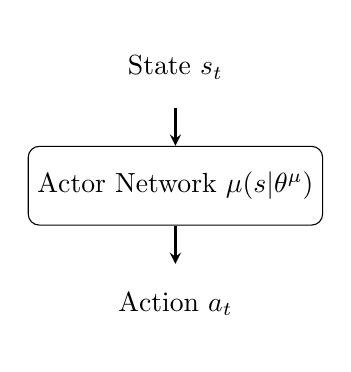
\begin{tikzpicture}
			[node distance=1.5cm]
			\node[object] (state)  {State $s_t$ };
			\node[element, below of=state] (localActor){ Actor Network $\mu(s|\theta^\mu)$};
			\node[object, below of=localActor] (action){ Action $a_t$};
			
			\draw[arrow] (state) -- (localActor);
			\draw[arrow] (localActor) -- (action);
			\end{tikzpicture}
			\begin{tikzpicture}
			[node distance=1.5cm]
			\node[object, left of=action] (state)  {State $s_t$ };
			\node[object, right of=state] (action)  {Action $a_t$};
			\node[element,below = of $(state)!0.5!(action)$] (localCritic){ Critic Local $Q(s,a|\theta^Q)$};
			\node[object, below of=localCritic] (value){ Q-value $q_t$};
			
			\draw[arrow] (state) -- (localCritic);
			\draw[arrow] (action) -- (localCritic);
			\draw[arrow] (localCritic) -- (value);
			%\draw [draw, -latex',thick] (3.east) -- ++(2,0) node(lowerright){} |- (state.east);
			
			\end{tikzpicture}
		\end{center}		
		\caption{Actor and Critic Networks}
		\label{fig:actor_critic}
	\end{figure}
	In DDPG we have 4 neural networks: the \textbf{local Actor}, the \textbf{local Critic}, the \textbf{target Actor} and the \textbf{target Critic}. The aim of Actor networks is to approximate the \textbf{Policy} while the Critic networks approximate the \textbf{Q-Value}.
	
	Initially Actors and Critics have the same randomly initialized weights. Then the local Actor (the current policy) starts to propose actions to the Agent, given the current state, starting to populate the Replay Buffer of experiences.
	
	When the Replay Buffer is big enough, the algorithm starts to sample randomly a mini-batch of experiences for each timestep $t$. This mini-batch is used to update the local Critic minimizing the Mean Squared Loss between the local Q-value and the target one (\vref{eq9:loss}) and to update the actor policy using the sampled policy gradient (\vref{eq8:mean_gradient}).
	
	\begin{equation}\label{eq9:loss}
	L = \frac{1}{N} \sum_i(y_i -Q(s_i, a_i|\theta^Q))^2
	\end{equation}\label{eq10:gradient}
	where $y_i$ is given by \vref{eq5:yt}.
	
	We can imagine the target networks as the \textit{labels} of supervised learning.
	
	Also the target networks are updated in this \textit{learning step}. A mere copy of the local weights is not an efficient solution, because it is prone to divergence. For this reason, a "soft" target updates is used. It is given by \[\theta' \leftarrow \tau\theta' \leftarrow \tau \theta + (1-\tau)\theta'\] with $t \ll 1$.
	
	The pseudo-code of this procedure is shown in \vref{ddpgalg}
	
	\subsubsection{Exploration vs. Exploitation} 
	In Reinforcement learning for discrete action spaces, exploration is done selecting a random action (e.g.\ epsilon-greedy). For continuous action spaces, exploration is done adding noise to the action itself. In \cite{lillicrap2015continuous}, the authors use Ornstein-Uhlenbeck Process \cite{uhlenbeck1930theory} to add noise to the action output $
	a_t = \mu(s_t|\theta^\mu) + \mathcal{N}$. After that the action is clipped in the correct range.
	 
	\subsection{Steps made}
	The initial step was trying to implement the algorithm in \cite{lillicrap2015continuous} using two simple environment provided by OpenAI Gym: \textit{MountainCarContinuous-v0} and \textit{Pendulum-v0}. In this report we will use only shallow Neural Networks implemented as shown in \vref{fig:actor_critic_schema}, because the state is represented directly by the data of the observation.
	
	The next goal will be to apply a Convolutional Neural Network (CNN) to states represented by a set of RGB images of the same environments.
	
	In this report the algorithm was implemented using a simple Replay Buffer and a Prioritized one in order to understand better the efficiency and the differences. In \vref{results} is possible to observe the results and the comparison of these two approach.
	
	\subsubsection{Hyper Parameters}
	The aim of this section is to describe the Hyper Parameters of DDPG.
	
	\begin{description}
		\item[Epsilon (\texttt{eps\_start}, \texttt{eps\_end}, \texttt{eps\_decay})] it is described by the function \[\epsilon = \epsilon_{\text{start}} - (\epsilon_{\text{start}} -\epsilon_{\text{end}})\min(1.0, \frac{e}{\epsilon_{\text{decay}}})\] where $e$ is the current episode number. It is used to decrease the impact of the noise on the actions in function of the number of episode. When it reaches the \texttt{eps\_end}, it will become a constant.
		
		% \texttt{default: [eps\_start = 0.9, eps\_end = 0.2, eps\_decay = max\_episode]}
		
		\item[Noise (\texttt{mu}, \texttt{sigma}, \texttt{theta})] these are the Ornstein-Uhlenbeck Process Noise parameters.
		
		% \texttt{default: [mu = 0.0, sigma = 0.3, theta = 0.15]}
		
		\item[Replay (\texttt{batch\_size}, \texttt{replay\_min\_size}, \texttt{replay\_max\_size})] \texttt{batch\_size} is the dimension of the mini-batch sampled by the memory. The learning process starts when the replay memory contains at least \texttt{replay\_min\_size} transitions and it starts to overwrite old transitions when it reaches \texttt{replay\_max\_size}.
		
		% \texttt{default: [batch\_size = 100, replay\_min\_size = 10000, replay\_max\_size = 1000000]}
		
		\item[Episode (\texttt{n\_episode}, \texttt{episode\_max\_len})] the number of episode for each run is \texttt{n\_episode}, while the maximum length of an episode is \texttt{episode\_max\_len}.
		
		% \texttt{default: [n\_episode = 300-500, episode\_max\_len = 300-1000]}
		
		\item[Neural Networks (\texttt{weight\_decay}, \texttt{update\_method}, \texttt{lr})] set of parameter for each network. The first parameter is always set to 0 and never used. The second one is always set to Adaptive Moment Estimation (ADAM), while the third is the learning rate and it is usually set to \texttt{1e-3} or \texttt{1e-4}.
		
		% \texttt{default: [weight\_decay = 0, update\_method = 'adam', lr = 1e-3,1e-4]}
		
		\item[Update (\texttt{discount}, \texttt{soft\_target\_tau}, \texttt{n\_updates\_per\_step})] \texttt{discount} is $\gamma$, \texttt{soft\_target\_tau} is $\tau$, while \texttt{n\_updates\_per\_step} is the number of times that the algorithm has to extract a mini-batch and perform the update of the networks for each timestep.
		
		% \texttt{default: [discount = 0.99, soft\_target\_tau = 0.001, n\_updates\_per\_episode = 1]}
		
		\item[Test (\texttt{n\_tests}, \texttt{every\_n\_episode})] \texttt{n\_tests} is the number of episode to test in the testing phase, while \texttt{every\_n\_episode} indicates how often the testing phase starts. 
		
		% \texttt{default: [n\_tests = 10]}
		
		
	\end{description}
\begin{algorithm}[!h]
	\SetAlgoLined
	Randomly initialize critic network $Q(s,a|\theta^Q)$ and actor $\mu(s|\theta^\mu)$ with weights $\theta^Q$ and $\theta^\mu$\;
	
	Initialize target network $Q'$ and $\mu'$ with weights $\theta^{Q'} \leftarrow \theta^Q$, $\theta^{\mu'} \leftarrow \theta^\mu$\;
	\For{episode = 1, M}{
		Initialize or Reset a random process $\mathcal{N}$ for action exploration\;
		Reset the environment and receive the initial observation state $s_1$\;
		\For{t = 1, T}{
			Select action $a_t = \mu(s_t|\theta^\mu) + \mathcal{N}$ and \textit{clipping} it to the limit of the environment\;
			Execute action $a_t$ and obtain $(r_t, s_{t+1}, d_t) \equiv (\text{reward, next state, done flag})$\;
			Store transition $(s_t, a_t, r_t, s_{t+1}, d_t)$ in $\mathcal{R}$\;
			\If{$\mathcal{R}$ has at least $M$ samples}{
				Sample random minibatch of $N \ll M$ transitions $(s_t, a_t, r_t, s_{t+1}, d_t)$ from $\mathcal{R}$\;
				Set $y_i = r_i + \gamma (1-d_i) Q'(s_{i+1}, \mu'(s_{i+1}|\theta^{\mu'})|\theta^{Q'})$\;
				Update the critic by minimizing the loss: $L = \frac{1}{N} \sum_i(y_i -Q(s_i, a_i|\theta^Q))^2$\;
				Update the actor policy using the sampled policy gradient:
				\[\nabla_{\theta^\mu}J \approx \frac{1}{N}\sum_{i}^{}\nabla_a Q(s, a|\theta^Q)|_{s=s_i, a=\mu(s_i)}\nabla_{\theta^\mu}\mu(s|\theta^\mu)|_{s_i}\]
				Update the target networks:
				\[\theta^{Q'} \leftarrow \tau \theta^Q +(1-\tau)\theta^{Q'}\]
				\[\theta^{\mu'} \leftarrow \tau \theta^\mu +(1-\tau)\theta^{\mu'}\]
			}
		}
	}
	\caption{DDPG Algorithm}
	\label{ddpgalg}
\end{algorithm}
\begin{figure}[!h]
	\begin{center}
		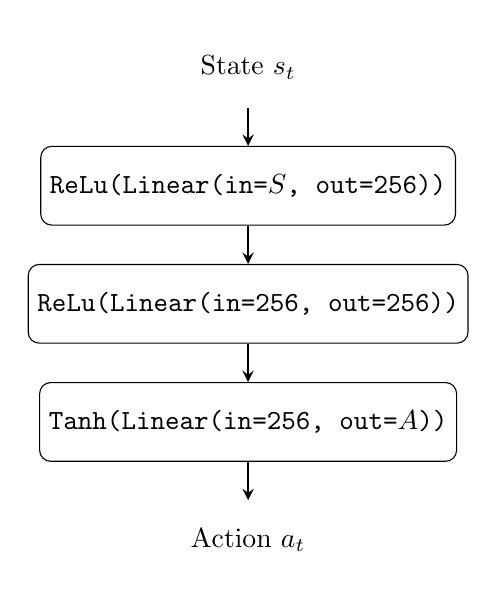
\begin{tikzpicture}
		[node distance=1.5cm]
		\node[object] (state)  {State $s_t$};
		\node[element, below of=state] (linear1){\texttt{ReLu(Linear(in=$S$, out=256))}
		};
		\node[element, below of=linear1] (linear2){\texttt{ReLu(Linear(in=256, out=256))}
		};
		\node[element, below of=linear2] (linear3){\texttt{Tanh(Linear(in=256, out=$A$))}
		};
		\node[object, below of=linear3] (action){ Action $a_t$};
		
		\draw[arrow] (state) -- (linear1);
		\draw[arrow] (linear1) -- (linear2);
		\draw[arrow] (linear2) -- (linear3);
		\draw[arrow] (linear3) -- (action);
		\end{tikzpicture}
		\begin{tikzpicture}
		[node distance=1.5cm]
		\node[object, left of=action] (state)  {State $s_t$ };
		\node[object, right of=state] (action)  {Action $a_t$};
		\node[element, below= of $(state)!0.5!(action)$] (linear1){\texttt{ReLu(Linear(in=$S+A$, out=256))}
		};
		\node[element, below of=linear1] (linear2){\texttt{ReLu(Linear(in=256, out=256))}
		};
		\node[element, below of=linear2] (linear3){\texttt{Linear(in=256, out=1)}
		};
		\node[object, below of=linear3] (value){ Q-value $q_t$};
		
		\draw[arrow] (state) -- (linear1);
		\draw[arrow] (action) -- (linear1);
		\draw[arrow] (linear1) -- (linear2);
		\draw[arrow] (linear2) -- (linear3);
		\draw[arrow] (linear3) -- (value);
		%\draw [draw, -latex',thick] (3.east) -- ++(2,0) node(lowerright){} |- (state.east);
		
		\end{tikzpicture}
	\end{center}		
	\caption{Actor and Critic Networks: $S$ is the length of the array of states, while $A$ is the length of the array of actions.}
	\label{fig:actor_critic_schema}
\end{figure}
	\section{OpenAI Gym Environments}
	\subsection{MountainCarContinuous-v0} 
	\subsubsection{Description}
	An underpowered car must climb a one-dimensional hill to reach a target. The action (engine force applied) is a continuous value. 
	The target is on top of a hill on the right-hand side of the car. If the car reaches it or goes beyond, the episode terminates. On the left-hand side, there is another hill. Climbing this hill can be used to gain potential energy and accelerate towards the target. On top of this second hill, the car cannot go further than a position equal to -1, as if there was a wall. Hitting this limit does not generate a penalty.
	%\begin{figure}[ht!]
	%	\centering
	%	\includegraphics[height=0.2\paperwidth]{img/mountaincar.png}
	%	\caption{Frame of MountainCarContinuous-v0 environment}
	%	\label{fig:mountaincar}
	%\end{figure}
	\paragraph{Observation}
	Type: Box(2)
	\begin{table}[!h]
		\centering
		% \caption{MountainCarContinuous-v0 Observation}
		\label{mountain_observation}
		\begin{tabular}{@{}lllll@{}}
			\toprule
			Index	& Observation		& Min 		& Max 		\\ \midrule
			0			& Car Position	 	&  $-1.2$	& $+0.6$ 	\\
			1			& Car Velocity	 	&  $-0.07$		& $+0.07$ \\
			\bottomrule
		\end{tabular}
	\end{table}
	\paragraph{Actions}
	Type: Box(1)
	\begin{table}[!h]
		\centering
		% \caption{MountainCarContinuous-v0 Actions }
		\label{mountain_action}
		\begin{tabular}{@{}lllll@{}}
			\toprule
			Index	& Action	& Min 		& Max 		\\ \midrule
			0			& Push car to the left (negative value) or to the right (positive value)&  $-1$	& $+1$ 	\\
			\bottomrule
		\end{tabular}
	\end{table}
	\paragraph{Reward}
	The reward for each timestep $t$ is given by $r_t = d_t*100 - a_t^2*0.1$
	where $d_t$ is the done flag and $a_t$ is the continuous value of the action taken.
	
	This reward function raises an exploration challenge, because if the agent does not reach the target soon enough, it will figure out that it is better not to move, and won't find the target anymore.
	
	\paragraph{Starting State}
	Position between -0.6 and -0.4, null velocity.
	\paragraph{Episode Termination}
	Position equal to 0.5.
	\paragraph{Solved Requirements}
	Get a reward over 90.
	
		\subsubsection{Hyper-Parameters Used}
	\begin{table}[!h]
		\centering
		% \caption{MountainCarContinuous-v0 Actions }
		\label{mountain_action}
		\begin{tabular}{@{}lllllll@{}}
			\toprule
		Type			&Parameter			& Value	& Parameter				& Value  & Parameter			&  Value 	\\		\midrule
		Epsilon & \texttt{eps\_start}	& $0.9$	&  \texttt{eps\_end}	& $0.2$ & \texttt{eps\_decay} 	& $300$		\\
		Noise & \texttt{mu}	& $0.0$	&  \texttt{sigma}	& $0.3$ & \texttt{theta} 	& $0.15$		\\
		Replay & \texttt{batch\_size}	& $100|32$	&  \texttt{replay\_min\_size}	& $10^4$ & \texttt{replay\_max\_size} 	& $10^6$		\\
		Episode & \texttt{n\_episode}	& $300$	&  \texttt{episode\_max\_len}	& $1000$ & 	& 		\\
		Networks & \texttt{weight\_decay}	& $0.0$	&  \texttt{update\_method}	& 'adam' & \texttt{lr} 	& $1e^{-4}$		\\
		Update & \texttt{discount}	& $0.99$	&  \texttt{soft\_target\_tau}	& $0.001$ & \texttt{n\_updates\_per\_step} 	& $1$		\\
		Test & \texttt{n\_tests}	& $100$	&  \texttt{every\_n\_episode}	& $10$ &  	& 	\\
		\bottomrule
		\end{tabular}
	\end{table}
	
	\subsection{Pendulum-v0} 
	\subsubsection{Description}
	The inverted pendulum swingup problem is a classic problem in the control literature. In this version of the problem, the pendulum starts in a random position, and the goal is to swing it up so it stays upright.
	%\begin{figure}[ht!]
	%	\centering
	%	\includegraphics[height=0.2\paperwidth]{img/pendulum.png}
	%	\caption{Frame of Pendulum-v0 environment}
	%	\label{fig:pendulum}
	%\end{figure}
	\paragraph{Observation}
	Type: Box(3)
	\begin{table}[!h]
		\centering
		% \caption{MountainCarContinuous-v0 Observation}
		\label{mountain_observation}
		\begin{tabular}{@{}lllll@{}}
			\toprule
			Index	& Observation		& Min 		& Max 		\\ \midrule
			0			& cos($\theta$)	 	&  $-1.0$	& $+1.0$ 	\\
			1			& sin($\theta$)	 	&  $-1.0$		& $+1.0$ \\
			2			& $\dot{\theta}$	 	&  $-8.0$		& $+8.0$ \\
			\bottomrule
		\end{tabular}
	\end{table}
	\paragraph{Actions}
	Type: Box(1)
	\begin{table}[!h]
		\centering
		% \caption{MountainCarContinuous-v0 Actions }
		\label{mountain_action}
		\begin{tabular}{@{}lllll@{}}
			\toprule
			Index	& Action	& Min 		& Max 		\\ \midrule
			0			& Joint effort &  $-2.0$	& $+2.0$ 	\\
			\bottomrule
		\end{tabular}
	\end{table}
	
	\paragraph{Reward}
	The reward for each timestep $t$ is given by \[r_t = -(\theta_t^2 + 0.1 \dot{\theta}^2 + 0.001 a_t^2)\]
	where theta is normalized between $-\pi$ and $\pi$. Therefore, the lowest cost is $-(\pi^2 + 0.1*8^2 + 0.001*2^2) = -16.2736044$, and the highest cost is $0$. In essence, the goal is to remain at zero angle (vertical), with the least rotational velocity, and the least effort.
	
	\paragraph{Starting State}
	Random angle from $-\pi$ to $\pi$, and random velocity between $-1$ and $1$
	\paragraph{Episode Termination}
	There is no specified termination. Adding a maximum number of steps might be a good idea. In this case 200.
	\paragraph{Solved Requirements}
	It is an unsolved environment, which means it does not have a specified reward threshold at which it is considered solved.
	
	\subsubsection{Hyper-Parameters Used}
	\begin{table}[!h]
		\centering
		% \caption{MountainCarContinuous-v0 Actions }
		\label{mountain_action}
		\begin{tabular}{@{}lllllll@{}}
			\toprule
			Type			&Parameter			& Value	& Parameter				& Value  & Parameter			&  Value 	\\		\midrule
			Epsilon & \texttt{eps\_start}	& $0.9$	&  \texttt{eps\_end}	& $0.2$ & \texttt{eps\_decay} 	& $300$		\\
			Noise & \texttt{mu}	& $0.0$	&  \texttt{sigma}	& $0.3$ & \texttt{theta} 	& $0.15$		\\
			Replay & \texttt{batch\_size}	& $30$	&  \texttt{replay\_min\_size}	& $2500$ & \texttt{replay\_max\_size} 	& $10^6$		\\
			Episode & \texttt{n\_episode}	& $300$	&  \texttt{episode\_max\_len}	& $200$ & 	& 		\\
			Networks & \texttt{weight\_decay}	& $0.0$	&  \texttt{update\_method}	& 'adam' & \texttt{lr} 	& $1e^{-4}$		\\
			Update & \texttt{discount}	& $0.99$	&  \texttt{soft\_target\_tau}	& $0.001$ & \texttt{n\_updates\_per\_step} 	& $1$		\\
			Test & \texttt{n\_tests}	& $100$	&  \texttt{every\_n\_episode}	& $10$ &  	& 	\\
			\bottomrule
		\end{tabular}
	\end{table}
	\newpage
	\section{Comparing Results} \label{results}
	
	In order to better evaluate the performances of these algorithms, \textbf{TensorboardX} was used. 
	The mean $\mu$, $min$,  $max$ and standard deviation $\sigma$ were calculated with a tool and the important areas they describe were plotted for better visualization.
	\paragraph{\color{train_color_2}{Training Phase}} The training phase was repeated 20 times for \texttt{n\_episode} episodes and the results were used to calculate aggregate values.
	\paragraph{\color{test_color_2}{Test Phase}} After \texttt{every\_n\_episode} episodes, the test phase was triggered. In this part the current actor network was set in evaluation mode and tested on 100 random episodes. Also these results were used to calculate aggregate values.
	
	In the first 10 episodes, the selection of the actions to take are sampled from a uniform random distribution over valid actions. This is a way to improve exploration in the first steps. After that, it returns to normal DDPG exploration.
	
	\subsection{Durations}
	\begin{table}[!h]
		\centering
		% \caption{MountainCarContinuous-v0 Actions }
		\label{mountain_action}
		\begin{tabular}{@{}lllllll@{}}
			\toprule
			Environment			&\multicolumn{2}{ c }{Uniform Replay Memory}	& \multicolumn{2}{ c }{Prioritized Replay Memory}\\		
			& One & Total & One & Total\\ \midrule
			MountainCarContinuous-v0	& 15 min	&  5 h	& 13 min & 4.5 h		\\
			Pendulum-v0	&  6 min	&  2 h	& 6 min & 2 h		\\
			\bottomrule
		\end{tabular}
	\end{table}
	
	\subsection{MountainCarContinuous-v0} \label{mountain}
	\subsubsection{Uniform Replay Memory} 
	\begin{figure}[h]
		\begin{tikzpicture}
		\begin{axis}[axis on top, 
		xmin=1,
		xmax=300,
		ymin=-50,
		ymax=100,
		height=\textheight*0.40,
		set layers=standard,
		cycle list name=train,
		grid=both,
		grid style={solid,gray!30!white},
		% axis lines=middle,
		xlabel=Episode,
		ylabel style={align=center}, ylabel=Reward Value,
		%legend style={at={(0.98,0.2)},anchor=east},
		legend pos=south east,
		 extra y ticks = {90},
		 	extra y tick style={grid=major, grid style={solid,green},y tick label style={
		 		/pgf/number format/.cd,precision=10
		}},
		% x label style={at={(axis description cs:0.5,0)},anchor=north},
		%y label style={at={(axis description cs:-0.1,.5)},rotate=90,anchor=south}
		]
		
		\addplot table[x=Step,y=Value, col sep=comma] {plot/replayBuffer/mountain-v0/train/episode/mean.csv};
		\addlegendentry{Mean $\mu$ Reward Episode};
		
		\addplot [name path=upper,draw=none, forget plot] table[x=Step,y expr=\thisrow{Max}, col sep=comma] {plot/replayBuffer/mountain-v0/train/episode/mean.csv};
		
		\addplot [name path=lower,draw=none, forget plot] table[x=Step,y expr=\thisrow{Min}, col sep=comma] {plot/replayBuffer/mountain-v0/train/episode/mean.csv};
		
		\addplot [fill=train_color_3] fill between[of=upper and lower];
		\addlegendentry{Area $[min, max]$};
		
		\addplot [name path=upper1,draw=none, area legend, forget plot] table[x=Step,y expr=\thisrow{Value}+\thisrow{Error}, col sep=comma] {plot/replayBuffer/mountain-v0/train/episode/mean.csv};
		
		\addplot [name path=lower1,draw=none, area legend, forget plot] table[x=Step,y expr=\thisrow{Value}-\thisrow{Error}, col sep=comma] {plot/replayBuffer/mountain-v0/train/episode/mean.csv};
		
		\addplot [fill=train_color_2] fill between[of=upper1 and lower1];
		\addlegendentry{Area $[\mu-\sigma, \mu+\sigma]$};

		
		
		\end{axis}
		\end{tikzpicture}
		\caption{Mean, Standard Deviation Range and Min-Max range of the reward of each episode over 20 runs. }
		\label{fig:mountain_r_train_episode}
	\end{figure}
	\begin{figure}[h]
		\begin{tikzpicture}
		\begin{axis}[axis on top, 
		xmin=1,
		xmax=300,
		ymin=-50,
		ymax=100,
		height=\textheight*0.40,
		set layers=standard,
		cycle list name=train,
		grid=both,
		grid style={solid,gray!30!white},
		% axis lines=middle,
		xlabel=Episode,
		ylabel style={align=center}, ylabel=Reward Value,
		%legend style={at={(0.98,0.2)},anchor=east},
		legend pos=south east,
		extra y ticks = {90},
		 	extra y tick style={grid=major, grid style={solid,green},y tick label style={
		 		/pgf/number format/.cd,precision=10
		}},
		% x label style={at={(axis description cs:0.5,0)},anchor=north},
		%y label style={at={(axis description cs:-0.1,.5)},rotate=90,anchor=south}
		]
		
		\addplot table[x=Step,y=Value, col sep=comma] {plot/replayBuffer/mountain-v0/train/meanLast100/mean.csv};
		%\addlegendentry{Mean Reward of last 100 episode};
		
		\addplot [name path=upper,draw=none, forget plot] table[x=Step,y expr=\thisrow{Max}, col sep=comma] {plot/replayBuffer/mountain-v0/train/meanLast100/mean.csv};
		
		\addplot [name path=lower,draw=none, forget plot] table[x=Step,y expr=\thisrow{Min}, col sep=comma] {plot/replayBuffer/mountain-v0/train/meanLast100/mean.csv};
		
		\addplot [fill=train_color_3] fill between[of=upper and lower];
		
		\addplot [name path=upper1,draw=none, forget plot] table[x=Step,y expr=\thisrow{Value}+\thisrow{Error}, col sep=comma] {plot/replayBuffer/mountain-v0/train/meanLast100/mean.csv};
		
		\addplot [name path=lower1,draw=none, forget plot] table[x=Step,y expr=\thisrow{Value}-\thisrow{Error}, col sep=comma] {plot/replayBuffer/mountain-v0/train/meanLast100/mean.csv};
		
		\addplot [fill=train_color_2] fill between[of=upper1 and lower1];
		
		\addlegendentry{Mean $\mu$ Reward Last 100};
		\addlegendentry{Area $[min, max]$};
		\addlegendentry{Area $[\mu-\sigma, \mu+\sigma]$};
		\end{axis}
		\end{tikzpicture}
		\caption{Mean, Standard Deviation Range and Min-Max range of the running reward mean of the last 100 episodes for each episode over 20 runs.}
		\label{fig:mountain_r_train_mean}
	\end{figure}
	\begin{figure}[h]
		\begin{tikzpicture}
		\begin{axis}[axis on top, 
		xmin=10,
		xmax=300,
		ymin=-50,
		ymax=100,
		height=\textheight*0.40,
		set layers=standard,
		cycle list name=test,
		grid=both,
		grid style={solid,gray!30!white},
		% axis lines=middle,
		xlabel=Episode,
		ylabel style={align=center}, ylabel=Reward Value,
		%legend style={at={(0.98,0.2)},anchor=east},
		legend pos=south east,
		 extra y ticks = {90},
		 	extra y tick style={grid=major, grid style={solid,green},y tick label style={
		 		/pgf/number format/.cd,precision=10
		}},
		% x label style={at={(axis description cs:0.5,0)},anchor=north},
		%y label style={at={(axis description cs:-0.1,.5)},rotate=90,anchor=south}
		]
		
		\addplot table[x=Step,y=Value, col sep=comma, fill=test_color_1] {plot/replayBuffer/mountain-v0/test/rewardMean/mean.csv};
		%\addlegendentry{Mean Reward of last 100 episode};
		
		\addplot [name path=upper,draw=none, forget plot] table[x=Step,y expr=\thisrow{Max}, col sep=comma] {plot/replayBuffer/mountain-v0/test/rewardMean/mean.csv};
		
		\addplot [name path=lower,draw=none, forget plot] table[x=Step,y expr=\thisrow{Min}, col sep=comma] {plot/replayBuffer/mountain-v0/test/rewardMean/mean.csv};
		
		\addplot [fill=test_color_3] fill between[of=upper and lower];
		
		\addplot [name path=upper1,draw=none, forget plot] table[x=Step,y expr=\thisrow{Value}+\thisrow{Error}, col sep=comma] {plot/replayBuffer/mountain-v0/test/rewardMean/mean.csv};
		
		\addplot [name path=lower1,draw=none, forget plot] table[x=Step,y expr=\thisrow{Value}-\thisrow{Error}, col sep=comma] {plot/replayBuffer/mountain-v0/test/rewardMean/mean.csv};
		
		\addplot [fill=test_color_2] fill between[of=upper1 and lower1];
		
		\addlegendentry{Mean $\mu$ Test Reward};
		\addlegendentry{Area $[min, max]$};
		\addlegendentry{Area $[\mu-\sigma, \mu+\sigma]$};
		
		
		\end{axis}
		\end{tikzpicture}
		\caption{Mean, Standard Deviation Range and Min-Max range of reward mean of the test phase (every 10 episodes) over 20 runs.}
		\label{fig:mountain_r_test}
	\end{figure}
	\begin{figure}[h]
		\begin{tikzpicture}
		\begin{axis}[axis on top, 
		xmin=10,
		xmax=300,
		ymin=0,
		ymax=1000,
		height=\textheight*0.40,
		set layers=standard,
		cycle list name=test,
		grid=both,
		grid style={solid,gray!30!white},
		% axis lines=middle,
		xlabel=Episode,
		ylabel style={align=center}, ylabel=Reward Value,
		%legend style={at={(0.98,0.2)},anchor=east},
		legend pos=north east,
		%extra y ticks = {90},
		%extra y tick style={grid=major, grid style={solid,green},y tick label style={
		%		/pgf/number format/.cd,precision=10
		%}},
		% x label style={at={(axis description cs:0.5,0)},anchor=north},
		%y label style={at={(axis description cs:-0.1,.5)},rotate=90,anchor=south}
		]
		
		\addplot table[x=Step,y=Value, col sep=comma, fill=test_color_1] {plot/replayBuffer/mountain-v0/test/steps/mean.csv};
		%\addlegendentry{Mean Reward of last 100 episode};
		
		\addplot [name path=upper,draw=none, forget plot] table[x=Step,y expr=\thisrow{Max}, col sep=comma] {plot/replayBuffer/mountain-v0/test/steps/mean.csv};
		
		\addplot [name path=lower,draw=none, forget plot] table[x=Step,y expr=\thisrow{Min}, col sep=comma] {plot/replayBuffer/mountain-v0/test/steps/mean.csv};
		
		\addplot [fill=test_color_3] fill between[of=upper and lower];
		
		\addplot [name path=upper1,draw=none, forget plot] table[x=Step,y expr=\thisrow{Value}+\thisrow{Error}, col sep=comma] {plot/replayBuffer/mountain-v0/test/steps/mean.csv};
		
		\addplot [name path=lower1,draw=none, forget plot] table[x=Step,y expr=\thisrow{Value}-\thisrow{Error}, col sep=comma] {plot/replayBuffer/mountain-v0/test/steps/mean.csv};
		
		\addplot [fill=test_color_2] fill between[of=upper1 and lower1];
		
		\addlegendentry{Mean $\mu$ Test Step};
		\addlegendentry{Area $[min, max]$};
		\addlegendentry{Area $[\mu-\sigma, \mu+\sigma]$};
		
		
		\end{axis}
		\end{tikzpicture}
		\caption{Mean, Standard Deviation Range and Min-Max range of the number of steps in the test phase (every 10 episodes) over 20 runs.}
		\label{fig:mountain_r_test_step}
	\end{figure}
	\FloatBarrier
	\subsubsection{Prioritized Replay Memory} 
	In this case the size of the mini-batch was reduced from 100 to 32 in order to make the learning faster.
	\begin{figure}[H]
		\begin{tikzpicture}
		\begin{axis}[axis on top, 
		xmin=1,
		xmax=300,
		ymin=-50,
		ymax=100,
		height=\textheight*0.40,
		set layers=standard,
		cycle list name=train,
		grid=both,
		grid style={solid,gray!30!white},
		% axis lines=middle,
		xlabel=Episode,
		ylabel style={align=center}, ylabel=Reward Value,
		%legend style={at={(0.98,0.2)},anchor=east},
		legend pos=south east,
		extra y ticks = {90},
		extra y tick style={grid=major, grid style={solid,green},y tick label style={
				/pgf/number format/.cd,precision=10
		}},
		% x label style={at={(axis description cs:0.5,0)},anchor=north},
		%y label style={at={(axis description cs:-0.1,.5)},rotate=90,anchor=south}
		]
		
		\addplot table[x=Step,y=Value, col sep=comma] {plot/prioritized/mountain-v0/train/episode/mean.csv};
		\addlegendentry{Mean $\mu$ Reward Episode};
		
		\addplot [name path=upper,draw=none, forget plot] table[x=Step,y expr=\thisrow{Max}, col sep=comma] {plot/prioritized/mountain-v0/train/episode/mean.csv};
		
		\addplot [name path=lower,draw=none, forget plot] table[x=Step,y expr=\thisrow{Min}, col sep=comma] {plot/prioritized/mountain-v0/train/episode/mean.csv};
		
		\addplot [fill=train_color_3] fill between[of=upper and lower];
		\addlegendentry{Area $[min, max]$};
		
		\addplot [name path=upper1,draw=none, area legend, forget plot] table[x=Step,y expr=\thisrow{Value}+\thisrow{Error}, col sep=comma] {plot/prioritized/mountain-v0/train/episode/mean.csv};
		
		\addplot [name path=lower1,draw=none, area legend, forget plot] table[x=Step,y expr=\thisrow{Value}-\thisrow{Error}, col sep=comma] {plot/prioritized/mountain-v0/train/episode/mean.csv};
		
		\addplot [fill=train_color_2] fill between[of=upper1 and lower1];
		\addlegendentry{Area $[\mu-\sigma, \mu+\sigma]$};
		
		
		
		\end{axis}
		\end{tikzpicture}
		\caption{Mean, Standard Deviation Range and Min-Max range of the reward of each episode over 20 runs. }
		\label{fig:mountain_p_train_episode}
	%\end{figure}
	%\begin{figure}[h]
		\begin{tikzpicture}
		\begin{axis}[axis on top, 
		xmin=1,
		xmax=300,
		ymin=-50,
		ymax=100,
		height=\textheight*0.40,
		set layers=standard,
		cycle list name=train,
		grid=both,
		grid style={solid,gray!30!white},
		% axis lines=middle,
		xlabel=Episode,
		ylabel style={align=center}, ylabel=Reward Value,
		%legend style={at={(0.98,0.2)},anchor=east},
		legend pos=south east,
		extra y ticks = {90},
		extra y tick style={grid=major, grid style={solid,green},y tick label style={
				/pgf/number format/.cd,precision=10
		}},
		% x label style={at={(axis description cs:0.5,0)},anchor=north},
		%y label style={at={(axis description cs:-0.1,.5)},rotate=90,anchor=south}
		]
		
		\addplot table[x=Step,y=Value, col sep=comma] {plot/prioritized/mountain-v0/train/meanLast100/mean.csv};
		%\addlegendentry{Mean Reward of last 100 episode};
		
		\addplot [name path=upper,draw=none, forget plot] table[x=Step,y expr=\thisrow{Max}, col sep=comma] {plot/prioritized/mountain-v0/train/meanLast100/mean.csv};
		
		\addplot [name path=lower,draw=none, forget plot] table[x=Step,y expr=\thisrow{Min}, col sep=comma] {plot/prioritized/mountain-v0/train/meanLast100/mean.csv};
		
		\addplot [fill=train_color_3] fill between[of=upper and lower];
		
		\addplot [name path=upper1,draw=none, forget plot] table[x=Step,y expr=\thisrow{Value}+\thisrow{Error}, col sep=comma] {plot/prioritized/mountain-v0/train/meanLast100/mean.csv};
		
		\addplot [name path=lower1,draw=none, forget plot] table[x=Step,y expr=\thisrow{Value}-\thisrow{Error}, col sep=comma] {plot/prioritized/mountain-v0/train/meanLast100/mean.csv};
		
		\addplot [fill=train_color_2] fill between[of=upper1 and lower1];
		
		\addlegendentry{Mean $\mu$ Reward Last 100};
		\addlegendentry{Area $[min, max]$};
		\addlegendentry{Area $[\mu-\sigma, \mu+\sigma]$};
		\end{axis}
		
		\end{tikzpicture}
		\caption{Mean, Standard Deviation Range and Min-Max range of the running reward mean of the last 100 episodes for each episode over 20 runs.}
		\label{fig:mountain_p_train_mean}
		\end{figure}
		\begin{figure}[h]
		\begin{tikzpicture}
		\begin{axis}[axis on top, 
		xmin=10,
		xmax=300,
		ymin=-50,
		ymax=100,
		height=\textheight*0.4,
		set layers=standard,
		cycle list name=test,
		grid=both,
		grid style={solid,gray!30!white},
		% axis lines=middle,
		xlabel=Episode,
		ylabel style={align=center}, ylabel=Reward Value,
		%legend style={at={(0.98,0.2)},anchor=east},
		legend pos=south east,
		extra y ticks = {90},
		extra y tick style={grid=major, grid style={solid,green},y tick label style={
				/pgf/number format/.cd,precision=10
		}},
		% x label style={at={(axis description cs:0.5,0)},anchor=north},
		%y label style={at={(axis description cs:-0.1,.5)},rotate=90,anchor=south}
		]
		
		\addplot table[x=Step,y=Value, col sep=comma, fill=test_color_1] {plot/prioritized/mountain-v0/test/rewardMean/mean.csv};
		%\addlegendentry{Mean Reward of last 100 episode};
		
		\addplot [name path=upper,draw=none, forget plot] table[x=Step,y expr=\thisrow{Max}, col sep=comma] {plot/prioritized/mountain-v0/test/rewardMean/mean.csv};
		
		\addplot [name path=lower,draw=none, forget plot] table[x=Step,y expr=\thisrow{Min}, col sep=comma] {plot/prioritized/mountain-v0/test/rewardMean/mean.csv};
		
		\addplot [fill=test_color_3] fill between[of=upper and lower];
		
		\addplot [name path=upper1,draw=none, forget plot] table[x=Step,y expr=\thisrow{Value}+\thisrow{Error}, col sep=comma] {plot/prioritized/mountain-v0/test/rewardMean/mean.csv};
		
		\addplot [name path=lower1,draw=none, forget plot] table[x=Step,y expr=\thisrow{Value}-\thisrow{Error}, col sep=comma] {plot/prioritized/mountain-v0/test/rewardMean/mean.csv};
		
		\addplot [fill=test_color_2] fill between[of=upper1 and lower1];
		
		\addlegendentry{Mean $\mu$ Test Reward};
		\addlegendentry{Area $[min, max]$};
		\addlegendentry{Area $[\mu-\sigma, \mu+\sigma]$};
		
		
		\end{axis}
		\end{tikzpicture}
		\caption{Mean, Standard Deviation Range and Min-Max range of reward mean of the test phase (every 10 episodes) over 20 runs.}
		\label{fig:mountain_p_test}
	\end{figure}
	\begin{figure}[!h]
		\begin{tikzpicture}
		\begin{axis}[axis on top, 
		xmin=10,
		xmax=300,
		ymin=0,
		ymax=1000,
		height=\textheight*0.45,
		set layers=standard,
		cycle list name=test,
		grid=both,
		grid style={solid,gray!30!white},
		% axis lines=middle,
		xlabel=Episode,
		ylabel style={align=center}, ylabel=Reward Value,
		%legend style={at={(0.98,0.2)},anchor=east},
		legend pos=north east,
		%extra y ticks = {90},
		%extra y tick style={grid=major, grid style={solid,green},y tick label style={
		%		/pgf/number format/.cd,precision=10
		%}},
		% x label style={at={(axis description cs:0.5,0)},anchor=north},
		%y label style={at={(axis description cs:-0.1,.5)},rotate=90,anchor=south}
		]
		
		\addplot table[x=Step,y=Value, col sep=comma, fill=test_color_1] {plot/prioritized/mountain-v0/test/steps/mean.csv};
		%\addlegendentry{Mean Reward of last 100 episode};
		
		\addplot [name path=upper,draw=none, forget plot] table[x=Step,y expr=\thisrow{Max}, col sep=comma] {plot/prioritized/mountain-v0/test/steps/mean.csv};
		
		\addplot [name path=lower,draw=none, forget plot] table[x=Step,y expr=\thisrow{Min}, col sep=comma] {plot/prioritized/mountain-v0/test/steps/mean.csv};
		
		\addplot [fill=test_color_3] fill between[of=upper and lower];
		
		\addplot [name path=upper1,draw=none, forget plot] table[x=Step,y expr=\thisrow{Value}+\thisrow{Error}, col sep=comma] {plot/prioritized/mountain-v0/test/steps/mean.csv};
		
		\addplot [name path=lower1,draw=none, forget plot] table[x=Step,y expr=\thisrow{Value}-\thisrow{Error}, col sep=comma] {plot/prioritized/mountain-v0/test/steps/mean.csv};
		
		\addplot [fill=test_color_2] fill between[of=upper1 and lower1];
		
		\addlegendentry{Mean $\mu$ Test Step};
		\addlegendentry{Area $[min, max]$};
		\addlegendentry{Area $[\mu-\sigma, \mu+\sigma]$};
		
		
		\end{axis}
		\end{tikzpicture}
		\caption{Mean, Standard Deviation Range and Min-Max range of the number of steps in the test phase (every 10 episodes) over 20 runs.}
		\label{fig:mountain_p_test_step}
	\end{figure}
	\FloatBarrier
	
	\subsection{Pendulum-v0}
	In this case the graph about the steps taken in the test phase is not useful, because all episodes took all 200 steps.
	\subsubsection{Uniform Replay Memory} 
	\begin{figure}[H]
		\begin{tikzpicture}
		\begin{axis}[axis on top, 
		xmin=1,
		xmax=200,
		ymin=-1800,
		ymax=0,
		height=\textheight*0.37,
		set layers=standard,
		cycle list name=train,
		grid=both,
		grid style={solid,gray!30!white},
		% axis lines=middle,
		xlabel=Episode,
		ylabel style={align=center}, ylabel=Reward Value,
		%legend style={at={(0.99,0.3)},anchor=east},
		legend pos=south east,
		% extra y ticks = {90},
	% 	extra y tick style={grid=major, grid style={solid,green},y tick label style={
		% 		/pgf/number format/.cd,precision=10
		%}},
		% x label style={at={(axis description cs:0.5,0)},anchor=north},
		%y label style={at={(axis description cs:-0.1,.5)},rotate=90,anchor=south}
		]
		
		\addplot table[x=Step,y=Value, col sep=comma] {plot/replayBuffer/pendulum-v0/train/episode/mean.csv};
		%\addlegendentry{Mean Reward of last 100 episode};
		
		\addplot [name path=upper,draw=none, forget plot] table[x=Step,y expr=\thisrow{Max}, col sep=comma] {plot/replayBuffer/pendulum-v0/train/episode/mean.csv};
		
		\addplot [name path=lower,draw=none, forget plot] table[x=Step,y expr=\thisrow{Min}, col sep=comma] {plot/replayBuffer/pendulum-v0/train/episode/mean.csv};
		
		\addplot [fill=train_color_3] fill between[of=upper and lower];
		
		\addplot [name path=upper1,draw=none, forget plot] table[x=Step,y expr=\thisrow{Value}+\thisrow{Error}, col sep=comma] {plot/replayBuffer/pendulum-v0/train/episode/mean.csv};
		
		\addplot [name path=lower1,draw=none, forget plot] table[x=Step,y expr=\thisrow{Value}-\thisrow{Error}, col sep=comma] {plot/replayBuffer/pendulum-v0/train/episode/mean.csv};
		
		\addplot [fill=train_color_2] fill between[of=upper1 and lower1];
		
		\addlegendentry{Mean $\mu$};
		\addlegendentry{Area $[min, max]$};
		\addlegendentry{Area $[\mu-\sigma, \mu+\sigma]$};
		
		\end{axis}
		\end{tikzpicture}
		\caption{Mean, Standard Deviation Range and Min-Max range of the reward of each episode over 20 runs.}
		\label{fig:pendulum_r_train_episode}
	%\end{figure}
	%\begin{figure}[H]
		\begin{tikzpicture}
		\begin{axis}[axis on top, 
		xmin=1,
		xmax=200,
		ymin=-1600,
		ymax=0,
		height=\textheight*0.37,
		set layers=standard,
		cycle list name=train,
		grid=both,
		grid style={solid,gray!30!white},
		% axis lines=middle,
		xlabel=Episode,
		ylabel style={align=center}, ylabel=Reward Value,
		%legend style={at={(0.99,0.3)},anchor=east},
		legend pos=south east,
		% extra y ticks = {90},
		% 	extra y tick style={grid=major, grid style={solid,green},y tick label style={
		% 		/pgf/number format/.cd,precision=10
		%}},
		% x label style={at={(axis description cs:0.5,0)},anchor=north},
		%y label style={at={(axis description cs:-0.1,.5)},rotate=90,anchor=south}
		]
		
		\addplot table[x=Step,y=Value, col sep=comma] {plot/replayBuffer/pendulum-v0/train/meanLast100/mean.csv};
		%\addlegendentry{Mean Reward of last 100 episode};
		
		\addplot [name path=upper,draw=none, forget plot] table[x=Step,y expr=\thisrow{Max}, col sep=comma] {plot/replayBuffer/pendulum-v0/train/meanLast100/mean.csv};
		
		\addplot [name path=lower,draw=none, forget plot] table[x=Step,y expr=\thisrow{Min}, col sep=comma] {plot/replayBuffer/pendulum-v0/train/meanLast100/mean.csv};
		
		\addplot [fill=train_color_3] fill between[of=upper and lower];
		
		\addplot [name path=upper1,draw=none, forget plot] table[x=Step,y expr=\thisrow{Value}+\thisrow{Error}, col sep=comma] {plot/replayBuffer/pendulum-v0/train/meanLast100/mean.csv};
		
		\addplot [name path=lower1,draw=none, forget plot] table[x=Step,y expr=\thisrow{Value}-\thisrow{Error}, col sep=comma] {plot/replayBuffer/pendulum-v0/train/meanLast100/mean.csv};
		
		\addplot [fill=train_color_2] fill between[of=upper1 and lower1];
		
		\addlegendentry{Mean $\mu$};
		\addlegendentry{Area $[min, max]$};
		\addlegendentry{Area $[\mu-\sigma, \mu+\sigma]$};
		
		\end{axis}
		\end{tikzpicture}
		\caption{Mean, Standard Deviation Range and Min-Max range of the running reward mean of the last 100 episodes for each episode over 20 runs.}
		\label{fig:pendulum_r_train_mean}
	\end{figure}
	\begin{figure}[H]
		\begin{tikzpicture}
		\begin{axis}[axis on top, 
		xmin=10,
		xmax=200,
		ymin=-1800,
		ymax=0,
		height=\textheight*0.40,
		set layers=standard,
		cycle list name=test,
		grid=both,
		grid style={solid,gray!30!white},
		% axis lines=middle,
		xlabel=Episode,
		ylabel style={align=center}, ylabel=Reward Value,
		%legend style={at={(0.99,0.3)},anchor=east},
		legend pos=south east,
		% extra y ticks = {90},
		% 	extra y tick style={grid=major, grid style={solid,green},y tick label style={
		% 		/pgf/number format/.cd,precision=10
		%}},
		% x label style={at={(axis description cs:0.5,0)},anchor=north},
		%y label style={at={(axis description cs:-0.1,.5)},rotate=90,anchor=south}
		]
		
		\addplot table[x=Step,y=Value, col sep=comma, fill=test_color_1] {plot/replayBuffer/pendulum-v0/test/rewardMean/mean.csv};
		%\addlegendentry{Mean Reward of last 100 episode};
		
		\addplot [name path=upper,draw=none, forget plot] table[x=Step,y expr=\thisrow{Max}, col sep=comma] {plot/replayBuffer/pendulum-v0/test/rewardMean/mean.csv};
		
		\addplot [name path=lower,draw=none, forget plot] table[x=Step,y expr=\thisrow{Min}, col sep=comma] {plot/replayBuffer/pendulum-v0/test/rewardMean/mean.csv};
		
		\addplot [fill=test_color_3] fill between[of=upper and lower];
		
		\addplot [name path=upper1,draw=none, forget plot] table[x=Step,y expr=\thisrow{Value}+\thisrow{Error}, col sep=comma] {plot/replayBuffer/pendulum-v0/test/rewardMean/mean.csv};
		
		\addplot [name path=lower1,draw=none, forget plot] table[x=Step,y expr=\thisrow{Value}-\thisrow{Error}, col sep=comma] {plot/replayBuffer/pendulum-v0/test/rewardMean/mean.csv};
		
		\addplot [fill=test_color_2] fill between[of=upper1 and lower1];
		
		\addlegendentry{Mean $\mu$};
		\addlegendentry{Area $[min, max]$};
		\addlegendentry{Area $[\mu-\sigma, \mu+\sigma]$};
		
		\end{axis}
		\end{tikzpicture}
		\caption{Mean, Standard Deviation Range and Min-Max range of reward mean of the test phase (every 10 episodes) over 20 runs.}
		\label{fig:pendulum_r_test}
	\end{figure}
	
	\FloatBarrier
	\subsubsection{Prioritized Replay Memory} \label{prioritized}
	\begin{figure}[!h]
		\begin{tikzpicture}
		\begin{axis}[axis on top, 
		xmin=1,
		xmax=200,
		ymin=-1800,
		ymax=0,
		height=\textheight*0.42,
		set layers=standard,
		cycle list name=train,
		grid=both,
		grid style={solid,gray!30!white},
		% axis lines=middle,
		xlabel=Episode,
		ylabel style={align=center}, ylabel=Reward Value,
		%legend style={at={(0.99,0.3)},anchor=east},
		legend pos=south east,
		% extra y ticks = {90},
		% 	extra y tick style={grid=major, grid style={solid,green},y tick label style={
		% 		/pgf/number format/.cd,precision=10
		%}},
		% x label style={at={(axis description cs:0.5,0)},anchor=north},
		%y label style={at={(axis description cs:-0.1,.5)},rotate=90,anchor=south}
		]
		
		\addplot table[x=Step,y=Value, col sep=comma] {plot/prioritized/pendulum-v0/train/episode/mean.csv};
		%\addlegendentry{Mean Reward of last 100 episode};
		
		\addplot [name path=upper,draw=none, forget plot] table[x=Step,y expr=\thisrow{Max}, col sep=comma] {plot/prioritized/pendulum-v0/train/episode/mean.csv};
		
		\addplot [name path=lower,draw=none, forget plot] table[x=Step,y expr=\thisrow{Min}, col sep=comma] {plot/prioritized/pendulum-v0/train/episode/mean.csv};
		
		\addplot [fill=train_color_3] fill between[of=upper and lower];
		
		\addplot [name path=upper1,draw=none, forget plot] table[x=Step,y expr=\thisrow{Value}+\thisrow{Error}, col sep=comma] {plot/prioritized/pendulum-v0/train/episode/mean.csv};
		
		\addplot [name path=lower1,draw=none, forget plot] table[x=Step,y expr=\thisrow{Value}-\thisrow{Error}, col sep=comma] {plot/prioritized/pendulum-v0/train/episode/mean.csv};
		
		\addplot [fill=train_color_2] fill between[of=upper1 and lower1];
		
		\addlegendentry{Mean $\mu$};
		\addlegendentry{Area $[min, max]$};
		\addlegendentry{Area $[\mu-\sigma, \mu+\sigma]$};
		
		\end{axis}
		\end{tikzpicture}
		\caption{Mean, Standard Deviation Range and Min-Max range of the reward of each episode over 20 runs.}
		\label{fig:pendulum_p_train_episode}
	\end{figure}
	\begin{figure}[!h]
		\begin{tikzpicture}
		\begin{axis}[axis on top, 
		xmin=1,
		xmax=200,
		ymin=-1600,
		ymax=0,
		height=\textheight*0.42,
		set layers=standard,
		cycle list name=train,
		grid=both,
		grid style={solid,gray!30!white},
		% axis lines=middle,
		xlabel=Episode,
		ylabel style={align=center}, ylabel=Reward Value,
		%legend style={at={(0.99,0.3)},anchor=east},
		legend pos=south east,
		% extra y ticks = {90},
		% 	extra y tick style={grid=major, grid style={solid,green},y tick label style={
		% 		/pgf/number format/.cd,precision=10
		%}},
		% x label style={at={(axis description cs:0.5,0)},anchor=north},
		%y label style={at={(axis description cs:-0.1,.5)},rotate=90,anchor=south}
		]
		
		\addplot table[x=Step,y=Value, col sep=comma] {plot/prioritized/pendulum-v0/train/meanLast100/mean.csv};
		%\addlegendentry{Mean Reward of last 100 episode};
		
		\addplot [name path=upper,draw=none, forget plot] table[x=Step,y expr=\thisrow{Max}, col sep=comma] {plot/prioritized/pendulum-v0/train/meanLast100/mean.csv};
		
		\addplot [name path=lower,draw=none, forget plot] table[x=Step,y expr=\thisrow{Min}, col sep=comma] {plot/prioritized/pendulum-v0/train/meanLast100/mean.csv};
		
		\addplot [fill=train_color_3] fill between[of=upper and lower];
		
		\addplot [name path=upper1,draw=none, forget plot] table[x=Step,y expr=\thisrow{Value}+\thisrow{Error}, col sep=comma] {plot/prioritized/pendulum-v0/train/meanLast100/mean.csv};
		
		\addplot [name path=lower1,draw=none, forget plot] table[x=Step,y expr=\thisrow{Value}-\thisrow{Error}, col sep=comma] {plot/prioritized/pendulum-v0/train/meanLast100/mean.csv};
		
		\addplot [fill=train_color_2] fill between[of=upper1 and lower1];
		
		\addlegendentry{Mean $\mu$};
		\addlegendentry{Area $[min, max]$};
		\addlegendentry{Area $[\mu-\sigma, \mu+\sigma]$};
		
		\end{axis}
		\end{tikzpicture}
		\caption{Mean, Standard Deviation Range and Min-Max range of the running reward mean of the last 100 episodes for each episode over 20 runs.}
		\label{fig:pendulum_p_train_mean}
	\end{figure}
\vfill
	\begin{figure}[!h]
		\begin{tikzpicture}
		\begin{axis}[axis on top, 
		xmin=10,
		xmax=200,
		ymin=-1800,
		ymax=0,
		height=\textheight*0.42,
		set layers=standard,
		cycle list name=test,
		grid=both,
		grid style={solid,gray!30!white},
		% axis lines=middle,
		xlabel=Episode,
		ylabel style={align=center}, ylabel=Reward Value,
		%legend style={at={(0.99,0.3)},anchor=east},
		legend pos=south east,
		% extra y ticks = {90},
		% 	extra y tick style={grid=major, grid style={solid,green},y tick label style={
		% 		/pgf/number format/.cd,precision=10
		%}},
		% x label style={at={(axis description cs:0.5,0)},anchor=north},
		%y label style={at={(axis description cs:-0.1,.5)},rotate=90,anchor=south}
		]
		
		\addplot table[x=Step,y=Value, col sep=comma, fill=test_color_1] {plot/prioritized/pendulum-v0/test/rewardMean/mean.csv};
		%\addlegendentry{Mean Reward of last 100 episode};
		
		\addplot [name path=upper,draw=none, forget plot] table[x=Step,y expr=\thisrow{Max}, col sep=comma] {plot/prioritized/pendulum-v0/test/rewardMean/mean.csv};
		
		\addplot [name path=lower,draw=none, forget plot] table[x=Step,y expr=\thisrow{Min}, col sep=comma] {plot/prioritized/pendulum-v0/test/rewardMean/mean.csv};
		
		\addplot [fill=test_color_3] fill between[of=upper and lower];
		
		\addplot [name path=upper1,draw=none, forget plot] table[x=Step,y expr=\thisrow{Value}+\thisrow{Error}, col sep=comma] {plot/prioritized/pendulum-v0/test/rewardMean/mean.csv};
		
		\addplot [name path=lower1,draw=none, forget plot] table[x=Step,y expr=\thisrow{Value}-\thisrow{Error}, col sep=comma] {plot/prioritized/pendulum-v0/test/rewardMean/mean.csv};
		
		\addplot [fill=test_color_2] fill between[of=upper1 and lower1];
		
		\addlegendentry{Mean $\mu$};
		\addlegendentry{Area $[min, max]$};
		\addlegendentry{Area $[\mu-\sigma, \mu+\sigma]$};
		
		\end{axis}
		\end{tikzpicture}
		\caption{Mean, Standard Deviation Range and Min-Max range of reward mean of the test phase (every 10 episodes) over 20 runs.}
		\label{fig:pendulum_p_test}
	\end{figure}
	\FloatBarrier
	
	\newpage
	\section{Comments} \label{final}
	
	Analyzing the graphs, it is clear that the results in moving from the Replay Buffer to the Prioritized Buffer are not as impressive as it was expected.
	
	The results obtained are almost the same or slightly better, on the other hand the execution time increases: for this reason the number of element extracted from the mini-batch at each episode was decreased.
	
	In the \textit{MountainCarContinuous-v0} environment, the mean on the last 100 episodes shown in \vref{fig:mountain_p_train_mean} is not better than \vref{fig:mountain_r_train_mean}, especially around 150th episode. But above the 260th episode the results are more stable and efficient.
	Also comparing the graphs of test phase, the results do not strongly improve.
	
	In the \textit{Pendulum-v0} environment the situation is overall the same, without any important improvement. In some cases the Uniform Replay Buffer seems more efficient in the first part, while the Prioritized one seems more stable in the last episodes.
	
	The aim of the Prioritized Buffer is to give more importance to surprising results. For this reason, I think that having worse results in the first part of the training (0-100 episodes) is normal and it is part of the algorithm. I expected impressive results in the last part, but unfortunately I obtained only slightly better results.
	
	I think that the problem may be caused by some bugs in the implementation of this part.
		
	\section{Next Steps} \label{next}
	The next steps that I am planning to analyze are:
	\begin{description}
		\item[Prioritized Problems] I think that the problem behind not impressive results of Prioritized Buffer are related to some bug in the implementation of this part. I will try to find a way to fix this.
		\item[Convolutional Neural Network] I had already started to test this part, but I have no relevant results, yet. I applied  the code to \textit{CarRacing-v0} which propose a continuous environment with a RGB vector as observation. I used a \texttt{StateBuffer} of size three to use the last three states as input for the Convolutional Neural Network ($9 \text{ inputs} = 3 \cdot 3 \text{ RGB channels}$).
		
		I found difficulties to test whether an algorithm or a particular CNN architecture is working because of the length of the training in this particular environment. I will try to find a better way to test: an idea could be to apply this approach to \textit{MountainCarConinuous-v0} or \textit{Pendulum-v0}, trying to get the image as observation instead of raw data.
		
		This is the \textbf{most important part} to develop because it is the base of the work with Anki Cozmo. I will focus mainly on that in the next days.
		
		\item[DDPG vs others] I am thinking to invest a part of the work in searching alternative algorithms recently discovered and reading new papers about them. For instance, some of the latest algorithm used in Autonomous Driving Reinforcement Learning are \textbf{Deep Distributed Distributional Deterministic Policy Gradients (D4PG)}, \textbf{Twin Delayed DDPG (TD3)} and \textbf{Soft Actor Critic (SAC)}. The last one is a sort of bridge between stochastic policy optimization and DDPG-style approaches. They seems promising in the context of the project and maybe they could lead to better results.
		I will try to explore more deeply this part.
		
	\end{description}	
	\newpage
	
	\bibliographystyle{unsrt}
	\bibliography{references}
	
\end{document}
